\chapter{Transformações Lineares}
Neste capítulo, iremos tratar sobre um tipo especial de função ou aplicação, onde, segundo \cite{steinbruch1987}, o domínio e o contradomínio são espaços vetoriais reais. Assim, tanto a variável independente como a variável dependente são vetores, razão pela qual essas funções são chamadas vetoriais.

Nosso estudo das funções vetoriais lineares em questão, será focado, nas transformações lineares.

\noindent\textbf{Definição 04:} Sejam $\mathbf{V}$ e $\mathbf{W}$ dois espaços vetoriais. Uma transformação linear (aplicação linear) é uma função de $\mathbf{V}$ em $\mathbf{W}$, $\mathbf{F}: \mathbf{V} \rightarrow \mathbf{W}$, que satisfaz as seguintes condições:

\begin{enumerate}
	\item Para quaisquer $\mathbf{u}$ e $\mathbf{v}$ em $\mathbf{V}$, $\mathbf{F}(\mathbf{u} + \mathbf{v}) = \mathbf{F}(u) + \mathbf{F}(v)$. \textbf{Homogeneidade}
	\item Para quaisquer $k \in \mathbb{R}$ e $\mathbf{v} \in \mathbf{V}$, $F(k\mathbf{v}) = k\mathbf{F}(\mathbf{v})$. \textbf{Aditividade}
\end{enumerate}	

No caso especial em que $\mathbf{V} = \mathbf{W}$, a transformação linear é denominada \textbf{operador linear} do espaço vetorial $\mathbf{V}$ \cite{anton2010elementary}.

\noindent\centerline{Válido em: $\forall \mathbf{v}, \mathbf{v} \in \mathbf{V}$ e $\forall k \in \mathbb{R}$. }

Trataremos $\mathbf{F}$ como $\mathbf{T}$ por convenção daqui em diante. Para se dizer que $\mathbf{T}$ é uma transformação linear do espaço vetorial $\mathbf{V}$ no espaço vetorial $\mathbf{W}$, será denotado por $\mathbf{T}:\mathbf{V}\longrightarrow\mathbf{W}$, onde $\mathbf{T}$ é a função, cada vetor $\mathbf{v} \in \mathbf{V}$ tem uma só imagem $\mathbf{w} \in \mathbf{W}$, indicado por $\mathbf{w} = \mathbf{T}(\mathbf{v})$.

Tomemos por dois conjuntos de vetores, $\mathbf{V} = \mathbb{R}^2$ e $\mathbf{W} = \mathbb{R}^3$.

Uma transformação de $\mathbf{T}:\mathbb{R}^2\longrightarrow\ \mathbb{R}^3$ associa vetores $\mathbf{v} = (x, y) \in \mathbb{R}^2$ com vetores $\mathbf{w} = (x, y, z) \in \mathbb{R}^3$

\noindent\textbf{Exemplo 11:} Declarado esta transformação linear $\mathbf{T}(x, y) = (x, y, x + y)$. Iremos selecionar alguns vetores em $\mathbb{R}^2$ e calcular suas imagens sob a transformação $\mathbf{T}$. Por exemplo, os vetores $(1, 0)$ e $(0, 1)$. Para $(1, 0)$, temos: 

\centerline{$\mathbf{T}(1, 0) = (1, 0, 1 +0) = (1, 0, 1)$}

\noindent e para $(0, 1)$, temos:

\centerline{$\mathbf{T}(0, 1) = (0, 1, 0 + 1) = (0, 1, 1)$.}

Segue a imagem em $\mathbb{R}^3$:

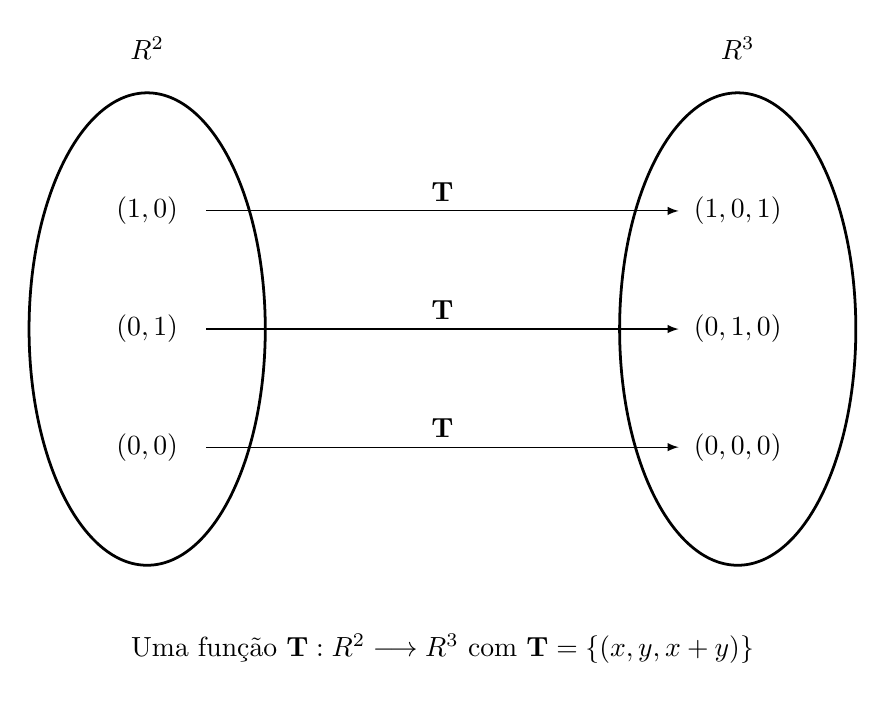
\begin{tikzpicture}[scale=1.5]
	\centering
	% Set A
	\draw[line width=1pt] (0,0) ellipse (1cm and 2cm);
	\node[above] at (0,2.2) (A) {$\mathbb{R}^2$};
	\node[centered] at (0,1) {$(1,0)$};
	\node[centered] at (0,0) {$(0,1)$};
	\node[centered] at (0,-1) {$(0,0)$};
	% Set B
	\draw[line width=1pt] (5,0) ellipse (1cm and 2cm);
	\node[above] at (5,2.2) (B) {$\mathbb{R}^3$};
	\node[centered] at (5,1) {$(1,0,1)$}; 
	\node[centered] at (5,0) {$(0,1,0)$};
	\node[centered] at (5,-1) {$(0,0,0)$};
	
	% Relations
	\draw[-latex, black] (0.5,1) -- node[midway, above] {$\mathbf{T}$} (4.5,1);
	\draw[-latex, black] (0.5, 0) -- node[midway, above] {$\mathbf{T}$} (4.5, 0);
	\draw[-latex, black] (0.5, -1) -- node[midway, above] {$\mathbf{T}$} (4.5, -1);
	
	% Label
	\node[below] at (2.5,-2.5) {Uma função $\mathbf{T}: \mathbb{R}^2 \longrightarrow \mathbb{R}^3$ com $\mathbf{T}=\{(x, y, x + y)\}$};
\end{tikzpicture}

\noindent\textbf{Exemplo 12:} Se tomarmos um vetor arbitrário e fazemos uma transformação linear idêntica, ou seja, $1\alpha$ = $\alpha$, é uma transformação linear de $\mathbf{V}$ em $\mathbf{V}$. A transformação é definida por $0\alpha = 0$, é também uma transformação linear de $\mathbf{V}$ em $\mathbf{V}$ \cite{hoffman1979}.

De acordo com o exemplo acima, percebe-se, que será uma função onde o gráfico passa a reta pela origem se supormos uma função afim, $\mathbb{R}^1$ em $\mathbb{R}^1$. Uma transformação linear mantém combinações lineares $W = [\mathbf{v}_1, \ldots, \mathbf{v}_n]$ são vetores que pertencem a $\mathbf{V}$ e possui seus escalares $c_1, \ldots, c_n$, então:

\centerline{$\mathbf{T}(c_1\mathbf{v}_1, \ldots, c_n\mathbf{v}_n) = \mathbf{T}(c_1\mathbf{v}_1 + c_2\mathbf{v}_2) = c_1(\mathbf{T}\mathbf{v}_1) + c_2(\mathbf{T}\mathbf{v}_2)$}

\noindent\textbf{Exemplo 13:} Tomemos um caso que desejamos dobrar nosso espaço vetorial, dado um vetor $\mathbf{V} = (2, 2); \mathbf{V} in \mathbb{R}^2$, a transformação linear será dada por, $\mathbf{T}(x, y) = (2x, 2y) in \mathbb{R}^2$. Nosso domínio e contradomínio está em $\mathbb{R}^2$, portanto o resultado será por $\mathbf{W} = (2 \times 2, 2 \times 2) \therefore \mathbf{W} = (4, 4)$

\begin{figure}[H]
	\centering
	\includegraphics[scale=1.30]{t_exemplo13.png}
	\caption{Exemplo 13.}
\end{figure}

Para uma matriz de transformação linear $\mathbf{T}$ de $\mathbf{V}$ em si mesma, existe uma matriz única $\mathbf{A}$ de dimensão $ n \times n$ que representa $\mathbf{T}$. Essa matriz é definida pela seguinte propriedade:

\centerline{$\mathbf{T}(\mathbf{v} = \mathbf{A}\mathbf{v})$}

\noindent para todo vetor $\mathbf{v}$ em $\mathbf{V}$. A matriz $\mathbf{A}$ é chamada de matriz de transformação de $\mathbf{T}$.

% Primeira aplicação citada da transforamação
Uma outra aplicação importante da transformação linear é no campo da geometria em uso de operações como rotações, reflexões e projeções. Considere o espaço vetorial bidimensional $\mathbb{R}^2$ com base canônica $\mathbf{e}_1 = (1, 0)$ e $\mathbf{e}_2 = (0, 1)$. A rotação de 90 graus no sentido anti-horário pode ser representada pela seguinte matriz de transformação:

\centerline{$\mathbf{R} = [[0, 1], [-1, 0]]$}

A matriz $\mathbf{R}$ chamada de matriz de rotação, possui algumas propriedades:

\begin{enumerate}
	\item \textbf{Ortogonalidade:} A matriz $\mathbf{R}$ é ortogonal, ou seja sua transporta é inversa:
	
	\centerline{$\mathbf{R}^T = \mathbf{R}^{-1}$}
	\item \textbf{Determinante:} O determinante da matriz $\mathbf{R}$ é igual a $-1$.
	
	\centerline{$\det(\mathbf{R}) = -1$}
\end{enumerate}

Ao rotacionar um vetor $\mathbf{v} = (x, y)$ em 90 graus  no sentido anti-horário, basta aplicar a matriz de rotação em $\mathbf{v}$.

\centerline{$\mathbf{v}' = \mathbf{R} \times \mathbf{v} = [[-1, 0], [0, -1]] \times [x, y] = [y, -x]$}

